%%This is a very basic article template.
%%There is just one section and two subsections.
\documentclass[a4paper,12pt]{article}
\usepackage[T2A]{fontenc} 
% \usepackage[cp1251]{inputenc}
\usepackage[utf8x]{inputenc}
\usepackage[english,russian]{babel}
\usepackage{amssymb,amsfonts,amsmath,mathtext,cite,enumerate,float}
\usepackage{hyperref}
\usepackage{cite}

\usepackage{indentfirst} 

\usepackage{graphicx} 
\graphicspath{{./img/}}

\usepackage{pstricks-add}

\usepackage{xcolor}
\newcommand\TODO[1]{\textcolor{red}{\textbf{TODO}: #1}}


\title{Современная экономическая система России} % Заглавие документа
\author{Фёдор Вомпе, 507 группа}
\date{\today} % Дата создания


\begin{document}

\maketitle

\section{Введение}

Несмотря на рецессию в 2009 году, среднегодовой темп роста экономики России за
последние 12 лет составил более 5\% в год\cite{TheEconomist}. По данным
Организации экономического сотрудничества и развития 
\footnote{ \textbf{Организация экономического сотрудничества
и развития} (сокр. ОЭСР, англ. Organization for Economic Co-operation and
Development, OECD) — международная экономическая организация развитых стран,
признающих принципы представительной демократии и свободной рыночной экономики.
- \textit{источник
\href{http://ru.wikipedia.org/wiki/Организация экономического сотрудничества
и развития}{Википедия}} } темпы роста экономики России замедлятся 
до 4\% в этом и следующем году\cite{StandardPoor}. В то время как инфляция может
вырасти по сравнению 6,1\% в прошлом году
% \footnote{По данным Росстата\cite{Rosstat} и журнала The
% Economist\cite{TheEconomist}}.
Уровень безработицы в настоящее время ниже среднего по данным ОЭСР.

В отличие от стойкого дефицита бюджета в 1990 году, за последние пару лет
в России наблюдается стойкий профицит бюджета. Все это благодаря
высокой и растущей цене за нефть, экономическому росту, а также
налоговой реформе.

Целью данной работы является анализ современной экономической
системы России, а также выявление основных экономических факторов, влияющих на
развитие экономики России. Основное внимание будет уделено структуре и динамике
ВВП России за последние несколько лет, т.к. в любой экономической системе
первичную роль играет производство в совокупности с распределением, обменом и потреблением.

\section{Структура экономики России и план её развития}

Рост реального ВВП России в 2011 году составил 4\% и может составить эту же
цифру в нынешнем году в связи c усилением рисков замедления роста мировой
экономики, вызванных замедлением роста экономик США и Евросоюза, а также 
затянувшегося долгового кризиса в Европе и ожидаемого снижения цен на
нефть. \cite{WorldBank2011} \\
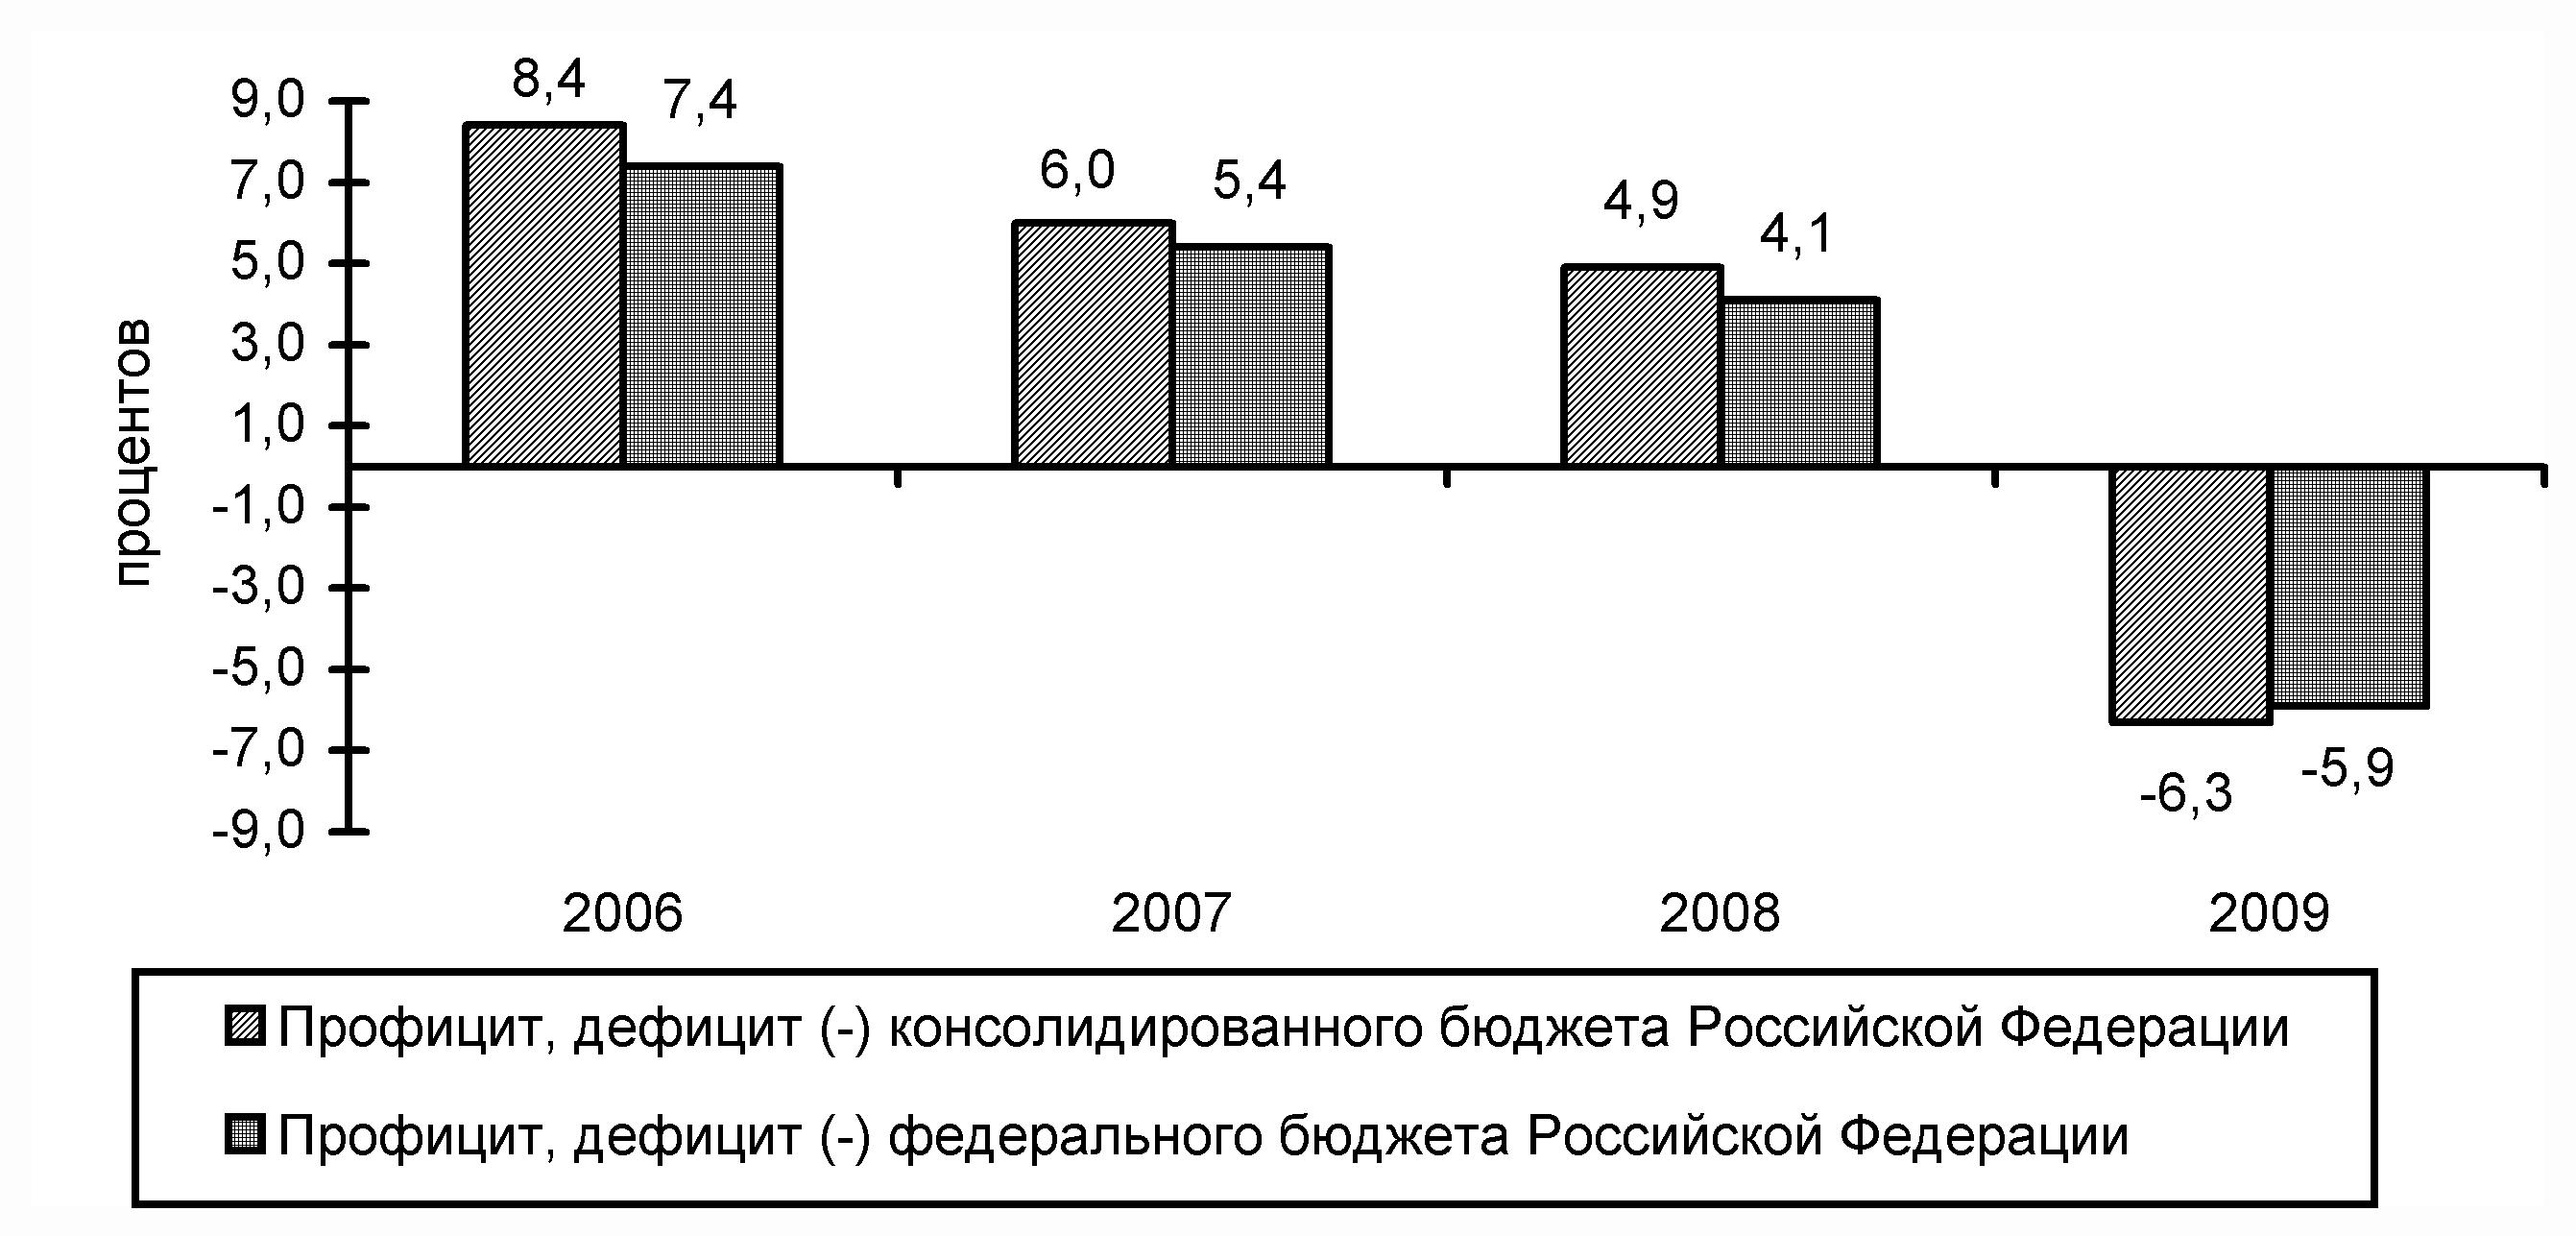
\includegraphics[width=1\textwidth]{Image3549.jpeg}
%По последним данным Росстата(на 2011 год) в структуре экономики России
%преобладает сектор услуг (торговля, транспорт, связь, финансовая деятельность,
%государственное управление, образование, здравоохранение, прочие слуги) 
%более 58,9 \% в ВВП. Этот показатель вырос примерно на 10\% с 2007 года.

Во время финансового кризиса 2009 года рост ВВП России составил отрицательную
величину -7.8\% по данным Всемирного банка в России и -6\% по данным Росстата.
Сельское хозяйство в 2010 рухнуло на 10\% по отношению к 2009 до минимумов с
2005. Единственный сектор, который не пострадал от экономического кризиса - это 
добывающая промышленность. Даже в кризис падения роста не было. Всего есть 6 
основных категорий, которые формируют ВВП России(в сумме 73.6\%
от ВВП) :
 добыча полезных ископаемых  (8.7\% от ВВП), 
 обрабатывающее производство (14.9\%), 
 розничная торговля (17.8\%), 
 транспорт (8.1\%), 
 операции с недвижимостью (9.2\%) и 
 налоги на продукты (14.9\%).

Среди всех отраслей промышленности России наиболее сильными, по отношению к 1991
году, являются: производство электрооборудования, электронного и оптического
оборудования, химическое производство, обрабатывающие производства, добыча топливно-энергетических полезных 
ископаемых; целлюлозно-бумажное производство (лесные ресурсы России — крупнейшие в мире); 
издательская и полиграфическая деятельность; металлургическое производство и производство 
готовых металлических изделий; производство и распределение электроэнергии, газа
и воды (по данным на 2011 год).

Для понимания дальнейшего развития экономической системы России надо ответить
на вопрос о роли и влиянии новейших технологий. 

Согласно теории отечественного экономиста Кондратьева Н.Д.\cite{Kondratiev},
научно-техническая революция развивается волнообразно, с циклами протяжённостью примерно в 50 лет. 
К настоящему времени известно пять технологических укладов (волн)\footnote{
\textbf{Технологический уклад(технологическая волна, tenor of technology)} — понятие теории
научно-технического прогресса, введенное в науку отечественными экономистами Д. С. Львовым и С. Ю. Глазьевым: совокупность 
сопряженных производств (взаимосвязанных технологических цепей), имеющих единый 
технический уровень и рассматриваемых как некая структурная подсистема 
экономической системы — альтернативная по отношению к таким подсистемам, 
как отрасли. - \textit{ Экономико-математический словарь\cite{Lopatnikov}} }.

Первая волна (1785—1835) сформировала технологический уклад, основанный на
новых технологиях в текстильной промышленности, использовании энергии воды.

Вторая волна (1830—1890) — ускоренное развитие железнодорожного и водного
транспорта на основе паровых машин, широкое внедрение паровых двигателей в
промышленное производство.

Третья волна (1880—1940) — использование в промышленном производстве
электрической энергии, развитие тяжёлого машиностроения и электротехнической
промышленности на основе использования стального проката, новых открытий в
области химии. Распространение радиосвязи, телеграфа, развитие автомобильной
промышленности. Образование крупных фирм, картелей, синдикатов и трестов.
Господство монополий на рынках. Начало концентрации банковского и финансового
капитала.

Четвёртая волна (1930—1990) — формирование мирового уклада, основанного на
дальнейшем развитии энергетики с использованием нефти и нефтепродуктов, газа,
средств связи, новых синтетических материалов. Период массового производства
автомобилей, тракторов, самолётов, различных видов вооружения, товаров
народного потребления. Широкое распространение компьютеров и программных
продуктов. Использование атомной энергии в военных и мирных целях. Конвейерные
технологии становятся основой массовых производств. Образование 
транснациональных и межнациональных компаний, которые осуществляют прямые
инвестиции в рынки различных стран.

Сейчас идет пятая технологическая волна. Эта тема развита 
российскими экономистами Д.С. Львовым\cite{Lvov} и С.Ю.
Глазьевым\cite{Glaziev}): технология широко опирается на достижения в
области микроэлектроники, информатики, биотехнологии, генной инженерии, новых видов энергии, освоения космического пространства и т. п.
Происходит переход от разрозненных фирм к единой сети крупных и мелких компаний, 
соединенных электронной сетью на основе Интернета, осуществляющих тесное взаимодействие 
в области технологий, контроля качества продукции, планирования инноваций. Стоит
отметить, что по некоторым оценкам этот уклад начал формироваться в 1985 году и
будет продолжаться еще 50 лет.

Доля технологий пятого уклада в России составляет примерно 10\%, да и
то только в наиболее развитых отраслях: в военно-промышленном комплексе, в
авиакосмической промышленности. Более 50\% технологий относится к четвёртому
уровню, и около трети — к третьему. Отсюда понятна вся сложность стоящей
перед отечественной наукой и технологиями задачи: чтобы в течение ближайших 10 лет 
наша страна смогла войти в число государств с шестым технологическим укладом.

Это удастся только в том случае, если наука будет обладать
статусом самостоятельной отрасли экономики. Ведущие страны мира к этому уже пришли.  
Большинство из них активно развивает науку и систему
инноваций, своевременно внедряя достижения науки в производство.
\cite{SixthTechn}

\section{Заключение}

Таким образом для того, чтобы динамично развивались и другие отрасли экономики,
а не только добывающая промышленность, необходимо ввести дополнительные
стимулы для развития сфер образования, науки, новых технологий, а также отраслей
необходимых для полного перехода от прошедших технологических укладов к новейшему шестому укладу. 
Только изменение приоритетов в политике государства позволит укрепить и
модернизировать экономику России.

Три направления интеллектуальной деятельности - образование, наука и создание
высоких технологий - должны быть официально признаны важнейшими стратегическими
ресурсами развития России.

Первоочередной задачей является возрождение российской науки\cite{Yavlinsky} и
преодоление технологического отставания России. Необходимо улучшение
финансирования науки, разработка ключевых государственных приоритетов, 
пересмотр системы управления науки, преодоление кризиса кадров и привлечение
молодежи в науку, обеспечение связи науки с производством. Необходима
государственная поддержка высокотехнологичных отраслей промышленности:
аэрокосмической, отдельных сегментов машиностроения и ВПК, создание новых
конструкционных материалов. В то же время задача создания инфраструктуры
информационного общества требует опережающего развития микроэлектроники,
компьютерной и телекоммуникационной отраслей. Именно эти отрасли, развивающиеся
параллельно с проведением политики массовой компьютеризации, удешевления
мобильной связи, могут составить основу информационной индустрии, способной
стать главным фактором роста и конкурентоспособности российской экономики в будущем.


\bibliography{myrefs}{}   % expects file "myrefs.bib"
\bibliographystyle{unsrt} % (uses file "plain.bst")

\end{document}
